\documentclass[a4paper,12pt, titlepage]{article}
\usepackage{amssymb,amsthm,amsmath} %ams
\usepackage[finnish]{babel} %suomenkielinen tavutus
\usepackage[T1]{fontenc} %skanditavutus
\usepackage[utf8]{inputenc} % skandit utf-8 koodauksella

\usepackage{graphicx} %dokumentti sisältää eps-muotoisia kuvia

\usepackage{changepage}
\usepackage{array}
\usepackage{tabularx}

\usepackage{hyperref}
\hypersetup{
    colorlinks=false,
    pdfborder={0 0 0},
}

\usepackage{float}
\restylefloat{table}


\linespread{1.24} %riviväli 1.5
\sloppy % Vähentää tavutuksen tarvetta, "leventämällä" rivin keskellä olevia välilyöntejä.
\begin{document}

\begin{titlepage}
    \begin{center}
        \vspace*{1cm}
        
        \LARGE
        \textbf{Testausdokumentti}
        
        \vspace{0.5cm}
        \Large
        Aineopintojen harjoitustyö: Tietorakenteet ja algoritmit (alkukesä)
        
        \vspace{1.5cm}
        
        \large
        \textbf{Sami Korhonen} \\
        \text{014021868} \\
        \text{sami.korhonen@helsinki.fi}
        
		\vfill        
        \normalsize
        Tietojenkäsittelytieteen laitos\\
        Helsingin yliopisto\\
		\large        
        \today
        
    \end{center}
\end{titlepage}


%\tableofcontents
%\newpage

\section*{Ohjelman testaaminen}

\subsection*{Yksikkötestaaminen}
Ohjelmaa on pyritty testaamaan metoditasolla mahdollisimman kattavasti oleennaisten toimmallisuuksien osalta. Kaikista selkeimpiä seikkoja ei ole automaattisesti testattu, mutta konstruktoreiden, gettereiden ja settereiden virheet ovat tulleet vastaan ilman sen kummempaa testausta. 

Integraatiotestaamista ei ole puuhattu, eikä suurimpien metodien tarkka yksikkötestaaminenkaan ole välttämättä tarpeen, mikäli näiden toimivuus on hyvin ilmeistä ohjelmaa ajaessa.

\subsection*{Suoritustestaaminen}
Ohjelmaan on sisällytetty automaattisesti ajettavia laatikkosarjoja, ja kontteja, joita voidaan pakata testausmielessä. Näistä saadut tulokset tallennetaan tiedostoihin, joista ne voi kätevästi avata tarkasteltavaksi muissa ohjelmissa. Nämä ovat osoittautuneet hyödyllisiksi ohjelmaa kehittäessä ja optimoitaessa. Optimoinnin osalla olisi vielä työsarkaa jäljellä.

\section*{Testisyötteet}

Taulukossa [1] näkyy syötteet, jotka annettiin generaattorille testissä. Näiden lisäksi jokaisen testisetin kontin koko oli 6058x2438x2591 ja käytettävien laatikoiden yhteistilavuus oli 105\% kontin tilavuudesta
\begin{table}[H]
\begin{tabular}{r|c|c|c}
\textbf{Nimi}                      & \textbf{Tyyppien määrä} & \textbf{minX = minY = minZ} & \textbf{maxX = maxY = maxZ} \\
\hline
homo1                     & 1              & 20                 & 100                \\
homo2                     & 5              & 20                 & 100                \\
homo3                     & 20             & 20                 & 100                \\
homo4                     & 50             & 20                 & 100                \\
homo5                     & 100            & 20                 & 100                \\
homo6                     & 200            & 20                 & 100                \\
homo7                     & 400            & 20                 & 100                \\
homo8                     & 600            & 20                 & 100                \\
homo9                     & 800            & 20                 & 100                \\
homo10                    & 1000           & 20                 & 100                \\
\hline
koko1                     & 5              & 15                 & 20                 \\
koko2                     & 5              & 25                 & 30                 \\
koko3                     & 5              & 30                 & 50                 \\
koko4                     & 5              & 50                 & 80                 \\
koko5                     & 5              & 80                 & 100                \\
koko6                     & 5              & 100                & 120                \\
koko7                     & 5              & 120                & 160                \\
\hline
patukat                   & 5              & x, y = 10, z = 1000 & x, y = 30, z = 2000              
\end{tabular}
\caption{Generaattorin syötteet testattaessa}
\end{table}

\section*{Testien ajaminen}
Suoritustestaamisen testit voidaan ajaa tavallisesti ohjelmaa suorittaessa käyttäjälle ilmoitettavin komennoin. Tulokset tallennetaan tiedostoon, eikä niitä näytetä käyttäjälle ohjelmaa suorittaessa. Satunnaisgeneroituja testejä ei kannata ajaa kovin suurilla iteraatioiden määrällä, sillä tämä olisi aikaa vaativaa puuhaa, ja samalla riskeeraa tulosten menettämisen mahdollisten ylivuotojen seurauksena. 

Heikommilla tietokoneilla saattaa automaattiset testit keskeytyä muistin ylivuodon seurauksena. Tämän voisi välttää vaihtamalla sarjan "koko1" mitat suuremmiksi, jolloin laatikoita tulee pienempi määrä. Testit on ajettu tämänhetkistä sarjaa vaativammalla sarjalla.

\section*{Tulokset}
Tuloksista näkyy, että aikavaativuus riippuu hyvin paljon erityyppisten laatikoiden määrästä. Laatikoiden määrän vaikutus tulokseen alkaa näkyä vasta hyvin suurilla laatikoiden määrillä. Tässä testissä pienimmän sarjan "koko1" laatikoiden koko on hyvin pieni, jolloin laatikoita on täytynyt olla paljon, jotta kontin tilavuus saadaan täytettyä. Konttiin mahtuneiden laatikoiden tilavuuden suhde kontin tilavuuteen, eli täyttösuhde on yllättävän hyvä kaikilla sarjoilla. Alhaisimman tuloksen algoritmi sai hyvin heterogenisillä sarjoilla. Tämä on helppo selittää algoritmin yksinkertaisella tavalla rakentaa palkkeja, joka suoriutuu paremmin homogenisilla sarjoilla.

\begin{table}[h]
\begin{tabular}{r|c|c|c|c}
\textbf{nimi} & \textbf{Täyttösuhde} & \textbf{Aika(ms)} & \textbf{Laatikoiden määrä} & \textbf{Tyyppien määrä} \\
\hline
homo1         & 97,9279              & 25            & 51150                      & 1                       \\
homo2         & 99,4531              & 31            & 119243                     & 5                       \\
homo3         & 99,3940              & 143           & 180895                     & 20                      \\
homo4         & 97,8800              & 223           & 128195                     & 50                      \\
homo5         & 97,2845              & 452           & 142847                     & 100                     \\
homo6         & 91,2675              & 616           & 146011                     & 200                     \\
homo7         & 84,0248              & 883           & 118696                     & 400                     \\
homo8         & 76,7308              & 1182          & 102734                     & 600                     \\
homo9         & 73,9878              & 1587          & 92341                      & 800                     \\
homo10        & 75,9871              & 1915          & 111685                     & 1000                    \\
\hline
koko1         & 99,4615              & 10929         & 7946316                    & 5                       \\
koko2         & 99,3716              & 873           & 1790210                    & 5                       \\
koko3         & 99,4077              & 192           & 713743                     & 5                       \\
koko4         & 98,2434              & 14            & 138024                     & 5                       \\
koko5         & 98,0799              & 5             & 51513                      & 5                       \\
koko6         & 94,6598              & 3             & 27445                      & 5                       \\
koko7         & 94,2879              & 2             & 13574                      & 5                       \\
\hline
patukat       & 97,2762              & 8             & 71439                      & 5                      
\end{tabular}
\caption{Testin tulokset}
\end{table}

\begin{figure}[H]
  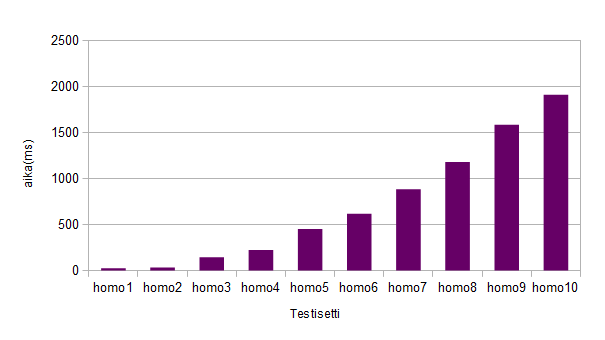
\includegraphics{homoaika.png}
  \caption{Homogeenisyyden vaikutus aikavaativuuteen}
\end{figure}
\begin{figure}[H]
  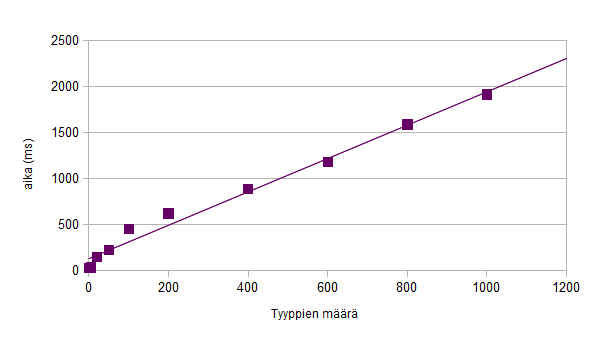
\includegraphics{tyyppiaika.png}
  \caption{Tyyppien määrän vaikutus aikavaativuuteen}
\end{figure}
\begin{figure}[H]
  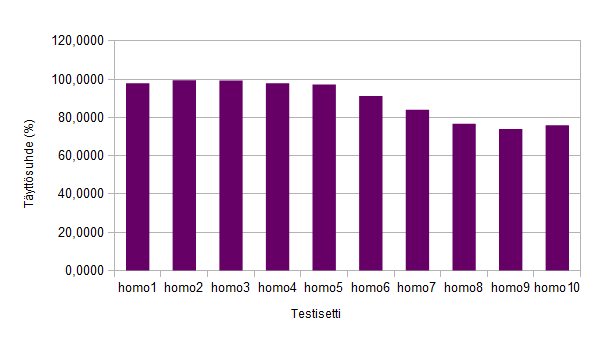
\includegraphics{homotaytto.png}
  \caption{Homogeenisyyden vaikutus täyttösuhteeseen}
\end{figure}
\begin{figure}[H]
  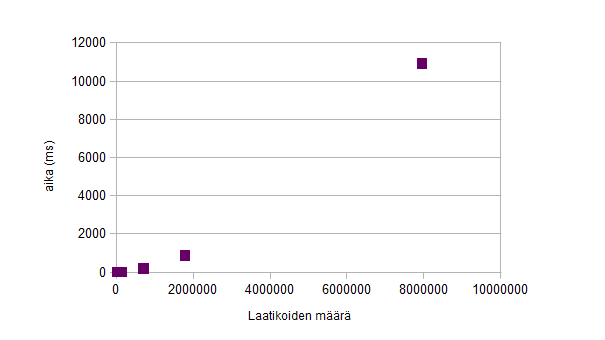
\includegraphics{maara-aika.png}
  \caption{Laatikoiden määrän vaikutus aikavaativuuteen}
\end{figure}


\end{document}
